\chapter{Funções do 2º grau}
As funções do 2º grau ou função quadrática são funções reais $f: \R \rightarrow \R$ dadas por:
\begin{equation*}
f(x)= ax^2 + bx + c \ ,
\end{equation*}
com $a, b, c \in \R$ e $a \neq 0$. 

O gráfico de uma função de 2º grau é um parábola. Nosso objetivo é extrair alguns elementos da função que possam nos orientar para representar seu gráfico com precisão.

Para determinar o gráfico, precisamos determinar quatro elementos importantes das parábolas que podem ser extraídas da função:

\begin{itemize}
    \item Concavidade: o gráfico da função de 2º grau tem concavidade voltada \textbf{para cima} quando \destaque{a > 0}, e concavidade voltada \textbf{para baixo} quando \destaque{a < 0}.
    
    \item Raízes: Os \textbf{zeros} ou \textbf{raízes} das funções de 2º grau $f$, quando existem, são os elementos $x$ de seu domínio tais que $ax^2+bx+c=0$. Por ser esta uma equação do 2º grau temos três situações a considerar, dependendo do valor de $\Delta=b^2-4ac$

 Se \destaque{\Delta < 0} a função $f$ não possui raízes reais;

 Se \destaque{\Delta = 0} a função $f$ possui uma única raiz real;

 Se \destaque{\Delta > 0} a função $f$ possui duas raízes reais distintas, que podem ser calculadas resolvendo a equação de 2º grau através da fórmula para equações de 2º grau.

 Por definição, os zeros da função $f(x)= ax^2+bx+c$, são as raízes da equação $ax^2+bx+c=0$, já que estes são os valores de $x$ para os quais $f(x)=0$. Graficamente, quando estas funções possuem zeros eles são exatamente os pontos de interseção do gráfico da $f$ com o eixo $x$.
 
    \item Interseção com o eixo $y$: esta inteseção ocorre quando $x=0$, ou seja, em $f(0)=c$.
    
    \item Vértice: a função do 2º grau possui um vértice dado pela seguinte equação:
\begin{equation*}
(x_V,y_V)= \left(\frac{- b}{2a}, \frac{- \Delta}{4a} \right).
\end{equation*}

 No caso em que $a > 0$, o vértice do gráfico da função de 2º grau é um ponto de mínimo da função.

 No caso em que $a < 0$, o vértice do gráfico da função de 2º grau é um ponto de máximo da função.
\end{itemize}
 
 \begin{exem}
 Considere a função $f(x)= x^2+x+1$. Observamos que:
 \begin{itemize}
     \item Esta função tem concavidade para cima pois $a=1$;
     \item A função $f$ não possui zeros pois $\Delta=-3$;
     \item Intersecta o eixo $y$ no ponto $(0,1)$;
     \item O vértice de $f$ é o ponto $(-\frac{1}{2}, \frac{3}{4})$.
 \end{itemize}

 % \begin{figure}[H]
 %  \centering
 %  \fbox{\includegraphics[height=5cm]{./cap_funcao/figs/f1}}
 %   \caption{Gráfico da função $f(x)= x^2+x+1$}
 %  \end{figure}

  \begin{center}
  \begin{tikzpicture}[scale=1]
    \tkzInit[xmin=-3, xmax=3, xstep=1, ymin=-1,ymax=4]
        %\tkzDrawXY
        \tkzAxeXY[fill=black!5]
        
        \tkzFct[thick,red]{x**2+x+1}
    
        %\tkzDefPointByFct[ref=A, with=a](-1)
        \tkzDefPoint(0,1){A}
        \tkzDefPoint(-0.5,0.75){B}
        \tkzPointShowCoord(B)
        \tkzDrawPoint[fill=red, size=3](A)
        \tkzDrawPoint[fill=red, size=3](B)
        
    \end{tikzpicture}
\end{center}
  
 \end{exem}
 
  \begin{exem}
 Considere a função $f(x)= x^2-4x+4$.
  %  \begin{figure}[H]
  % \centering
  % \fbox{\includegraphics[height=5cm]{./cap_funcao/figs/f2}}
  %  \caption{Gráfico da função $f(x)= x^2-4x+4$}
  % \end{figure}

\begin{itemize}
    \item Esta função tem concavidade para cima;
    \item O zero de $f$ é $S= \{2\}$;
    \item Intersecta o eixo $y$ no ponto $(0,4)$;
    \item O vértice de $f$ é o ponto $(2, 0)$.
\end{itemize}

\begin{center}
  \begin{tikzpicture}[scale=1]
    \tkzInit[xmin=-1, xmax=5, xstep=1, ymin=-1,ymax=5]
        %\tkzDrawXY
        \tkzAxeXY[fill=black!5]
        
        \tkzFct[thick,red]{x**2-4*x+4}
    
        %\tkzDefPointByFct[ref=A, with=a](-1)
        \tkzDefPoint(0,4){A}
        \tkzDefPoint(2,0){B}
        %\tkzPointShowCoord(A)
        \tkzDrawPoint[fill=red, size=3](A)
        \tkzDrawPoint[fill=red, size=3](B)
        
    \end{tikzpicture}
\end{center}
 \end{exem}
 
\begin{exem}
 Considere a função $f(x)= x^2-x-2$.

 \begin{itemize}
    \item Esta função tem concavidade para cima;
    \item As raízes de $f$ são $-1$ e $2$;
    \item Intersecta o eixo $y$ no ponto $(0,-2)$;
    \item O vértice de $f$ é o ponto $(\frac{1}{2}, -\frac{9}{4})$.
\end{itemize}

\begin{center}
  \begin{tikzpicture}[scale=1]
    \tkzInit[xmin=-3, xmax=3, xstep=1, ymin=-3,ymax=3]
        %\tkzDrawXY
        \tkzAxeXY[fill=black!5]
        
        \tkzFct[thick,red]{x**2-x-2}
    
        %\tkzDefPointByFct[ref=A, with=a](-1)
        \tkzDefPoint(0,-2){A}
        \tkzDefPoint(0.5,-2.25){B}
        \tkzPointShowCoord(B)
        \tkzDrawPoint[fill=red, size=3](A)
        \tkzDrawPoint[fill=red, size=3](B)
        
    \end{tikzpicture}
\end{center}
%    \begin{figure}[H]
%   \centering
%   \fbox{\includegraphics[height=5cm]{./cap_funcao/figs/f3}}
%    \caption{Gráfico da função $f(x)= x^2-x-2$}
%   \end{figure}
%  Observamos que:
%  \begin{enumerate}
% \item [a)] Os zeros de $f$ são $S= \{-1, 2\}$.
% \item [b)] O vértice de $f$ é o ponto $V= (0,5, -2,25)$.
% \item [c)] Esta função tem concavidade para cima.
% \item [d)] O vértice desta função é ponto de mínimo.
% \item [e)] A função é crescente no intervalo $(0,5, \infty)$.
% \item [f)] A função é decrescente no intervalo $(- \infty, 0,5)$.
% \end{enumerate}
\end{exem}

\begin{exem}
 Considere a função $f(x)= -x^2-x-2$.

 \begin{itemize}
    \item Esta função tem concavidade para baixo;
    \item A função $f$ não tem raiz real;
    \item Intersecta o eixo $y$ no ponto $(0,-2)$;
    \item O vértice de $f$ é o ponto $(-\frac{1}{2}, -\frac{7}{4})$.
\end{itemize}

\begin{center}
  \begin{tikzpicture}[scale=1]
    \tkzInit[xmin=-2, xmax=2, xstep=1, ymin=-4,ymax=1]
        %\tkzDrawXY
        \tkzAxeXY[fill=black!5]
        
        \tkzFct[thick,red]{-x**2-x-2}
    
        %\tkzDefPointByFct[ref=A, with=a](-1)
        \tkzDefPoint(0,-2){A}
        \tkzDefPoint(-0.5,-1.75){B}
        \tkzPointShowCoord(B)
        \tkzDrawPoint[fill=red, size=3](A)
        \tkzDrawPoint[fill=red, size=3](B)
        
    \end{tikzpicture}
\end{center}

%    \begin{figure}[H]
%   \centering
%   \fbox{\includegraphics[height=5cm]{./cap_funcao/figs/f4}}
%    \caption{Gráfico da função $f(x)= -x^2-x-2$}
%   \end{figure}
%  Observamos que:
%  \begin{enumerate}
% \item [a)] A função $f$ não possui zeros.
% \item [b)] O vértice de $f$ é o ponto $V= (-0,5, -1,75)$.
% \item [c)] Esta função tem concavidade para baixo.
% \item [d)] O vértice desta função é ponto de máximo.
% \item [e)] A função é crescente no intervalo $(- \infty, -0,5)$.
% \item [f)] A função é decrescente no intervalo $(-0,5, \infty)$.
% \end{enumerate}
\end{exem}

\begin{exem}
 Considere a função $f(x)= -x^2+6x-9$.

 \begin{itemize}
    \item Esta função tem concavidade para baixo;
    \item O zero de $f$ é $S= \{3\}$;
    \item Intersecta o eixo $y$ no ponto $(0,-9)$;
    \item O vértice de $f$ é o ponto $(3, 0)$.
\end{itemize}

\begin{center}
  \begin{tikzpicture}[scale=0.8]
    \tkzInit[xmin=-1, xmax=6, ymin=-9,ymax=1]
        %\tkzDrawXY
        \tkzAxeXY[fill=black!5]
        
        \tkzFct[thick,red,domain=0:6]{-x**2+6*x-9}
    
        %\tkzDefPointByFct[ref=A, with=a](-1)
        \tkzDefPoint(0,-9){A}
        \tkzDefPoint(3,0){B}
        %\tkzPointShowCoord(A)
        \tkzDrawPoint[fill=red, size=3](A)
        \tkzDrawPoint[fill=red, size=3](B)
        
    \end{tikzpicture}
\end{center}
%    \begin{figure}[H]
%   \centering
%   \fbox{\includegraphics[height=5cm]{./cap_funcao/figs/f5}}
%    \caption{Gráfico da função $f(x)= -x^2+6x-9$}
%   \end{figure}
%  Observamos que:
%  \begin{enumerate}
% \item [a)] O zero de $f$ é $S= \{3\}$.
% \item [b)] O vértice de $f$ é o ponto $V= (3, 0)$.
% \item [c)] Esta função tem concavidade para baixo.
% \item [d)] O vértice desta função é ponto de máximo.
% \item [e)] A função é crescente no intervalo $(-\infty, 3)$.
% \item [f)] A função é decrescente no intervalo $(3, \infty)$.
% \end{enumerate}
\end{exem}

\begin{exem}
 Considere a função $f(x)= -x^2+x+2$.

 \begin{itemize}
    \item Esta função tem concavidade para baixo;
    \item As raízes de $f$ são $-1$ e $2$;
    \item Intersecta o eixo $y$ no ponto $(0,2)$;
    \item O vértice de $f$ é o ponto $(\frac{1}{2}, \frac{9}{4})$.
\end{itemize}

\begin{center}
  \begin{tikzpicture}[scale=1]
    \tkzInit[xmin=-3, xmax=3, xstep=1, ymin=-3,ymax=3]
        %\tkzDrawXY
        \tkzAxeXY[fill=black!5]
        
        \tkzFct[thick,red]{-x**2+x+2}
    
        %\tkzDefPointByFct[ref=A, with=a](-1)
        \tkzDefPoint(0,2){A}
        \tkzDefPoint(0.5,2.25){B}
        \tkzPointShowCoord(B)
        \tkzDrawPoint[fill=red, size=3](A)
        \tkzDrawPoint[fill=red, size=3](B)
        
    \end{tikzpicture}
\end{center}

%    \begin{figure}[H]
%   \centering
%   \fbox{\includegraphics[height=5cm]{./cap_funcao/figs/f6}}
%    \caption{Gráfico da função $f(x)= -x^2+x+2$}
%   \end{figure}
%  Observamos que:
%  \begin{enumerate}
% \item [a)] Os zeros de $f$ são $S= \{-1, 2\}$.
% \item [b)] O vértice de $f$ é o ponto $V= (0,5, 2,25)$.
% \item [c)] Esta função tem concavidade para baixo.
% \item [d)] O vértice desta função é ponto de máximo.
% \item [e)] A função é crescente no intervalo $(-\infty, 0,5)$.
% \item [f)] A função é decrescente no intervalo $(0,5, \infty)$.
% \end{enumerate}
\end{exem}

% \begin{exem}
% Considere a função $f(x)= x^2 - 2x - 3$, determine:
% \begin{enumerate}
% \item [a)] Os zeros de $f$.
% \item [b)] O vértice de $f$.
% \item [c)] Esta função tem concavidade para cima ou para baixo?
% \item [d)] O vértice desta função é ponto de máximo ou mínimo?
% \item [e)] Qual o intervalo no qual a função é crescente?
% \item [f)] Qual o intervalo no qual a função é decrescente?
% \end{enumerate}
%   \begin{figure}[H]
%   \centering
%   \fbox{\includegraphics[height=5cm]{./cap_funcao/figs/funcao2grauexem1}}
%    \caption{Gráfico da função $f(x)= x^2 - 2x - 3$}
%   \end{figure}
% \end{exem}

% \begin{resol}
% \begin{enumerate}
% \item [a)] Os zeros de $f$ são $S= \{-1, 3\}$.
% \item [b)] O vértice de $f$ é o ponto $V= (1, -4)$.
% \item [c)] Esta função tem concavidade para cima.
% \item [d)] O vértice desta função é ponto de mínimo.
% \item [e)] A função é crescente no intervalo $(1, \infty)$.
% \item [f)] A função é decrescente no intervalo $(- \infty, 1)$.
% \end{enumerate}
% \end{resol}

% \begin{exem}
% Considere a função $f(x)= -x^2 + 2x + 8$, determine:
% \begin{enumerate}
% \item [a)] Os zeros de $f$.
% \item [b)] O vértice de $f$.
% \item [c)] Esta função tem concavidade para cima ou para baixo?
% \item [d)] O vértice desta função é ponto de máximo ou mínimo?
% \item [e)] Qual o intervalo no qual a função é crescente?
% \item [f)] Qual o intervalo no qual a função é decrescente?
% \end{enumerate}
%   \begin{figure}[H]
%   \centering
%   \fbox{\includegraphics[height=6cm]{./cap_funcao/figs/funcao2grauexem2}}
%    \caption{Gráfico da função $f(x)= -x^2 + 2x + 8$}
%   \end{figure}
% \end{exem}

% \begin{resol}
% \begin{enumerate}
% \item [a)] Os zeros de $f$ são $S= \{-2, 4\}$.
% \item [b)] O vértice de $f$ é o ponto $V= (1,9)$.
% \item [c)] Esta função tem concavidade voltada para baixo.
% \item [d)] O vértice desta função é ponto de máximo.
% \item [e)] A função é crescente no intervalo $(-\infty, 1)$.
% \item [f)] A função é decrescente no intervalo $(1, \infty)$.
% \end{enumerate}
% \end{resol}

\section{Máximos e mínimos da função de 2º grau}

    Seja $f:A\to \R$ uma função real.
\begin{itemize}
    \item Dizemos que $x_M\in A$ é ponto de máximo se $f(x_M)\geqslant f(x)$ para todo $x\in A$.

    \item Dizemos que $x_m\in A$ é ponto de mínimo se $f(x_m)\leqslant f(x)$ para todo $x\in A$.
\end{itemize}

\begin{teo}
    A função quadrática $f(x)=ax^2+bx+c$ admite um ponto de máximo $x_M$ se, e somente se, $a<0$.
\end{teo}

\begin{teo}
    A função quadrática $f(x)=ax^2+bx+c$ admite um ponto de mínimo $x_m$ se, e somente se, $a>0$.
\end{teo}

Com isto podemos determinar a imagem da função de 2º grau com domínio $\R$:
\begin{itemize}
    \item Se $a>0$ então a $\mathrm{Im}(f)=\left[y_V,+\infty)=[-\frac{\Delta}{4a},+\infty\right)$;
    \item Se $a<0$ então a $\mathrm{Im}(f)=\left(-\infty, y_V]=(-\infty,-\frac{\Delta}{4a}\right]$.
\end{itemize}

\begin{secExercicios}

\begin{exer}
    Esboce o gráfico das seguintes funções quadráticas $f:\R\to\R$:

    \begin{enumerate}[a)]
        \item $f(x)=x^2-3x+2$
        \item $f(x)=2x^2+3$
        \item $f(x)=-x^2+2x$
        \item $f(x)=-4x^2+4x-1$
        \item $f(x)=x^2-4$
        \item $f(x)=-x^2+4$
        \item $f(x)=x^2+2x+2$
        \item $f(x)=-x^2-4x-5$
    \end{enumerate}
\end{exer}

\begin{exer}
    Dadas as funções $f(x)=x^2-2x-3$, $g(x)=x^2-2x+1$ e $h(x)=x^2-2x+2$:
    \begin{enumerate}[a)]
        \item Obtenha os valores reais de $x$ tais que $f(x)=0$, $g(x)=0$ e $h(x)=0$.
        \item Dê o vértice de cada uma das parábolas;
        \item Esboce no mesmo sistema cartesiano os gráficos de $f$, $g$ e $h$.
    \end{enumerate}
\end{exer}

\begin{exer}
    Qual é o conjunto imagem de cada uma das funções?
    \begin{enumerate}[a)]
        \item $f(x)=-2x^2+4x-3$
        \item $f(x)=3x^2-5x+1$
    \end{enumerate}
\end{exer}

\begin{exer}
    Uma bola é lançada ao ar. Suponha que sua altura $h$, em metros, $t$ segundos após o lançamento, seja $h=-t^2+4t+6$. Determine:
    \begin{enumerate}[a)]
        \item o instante em que a bola atinge a sua altura máxima;
        \item a altura máxima atingida pela bola;
        \item quantos segundos depois do lançamento ela toca o solo.
    \end{enumerate}
\end{exer}

\begin{exer}
    Encontre a expressão da função quadrática $f:\R\to\R$ para cada um dos gráficos abaixo, justificando sua resposta:
    \begin{center}
        \begin{tikzpicture}[scale=1]
            \tkzInit[xmin=-1, xmax=5, xstep=1, ymin=-1,ymax=2]
            %\tkzDrawXY
            \tkzAxeXY
            
            \tkzFct[thick,red]{0.25*x**2-x+1}
        
            %\tkzDefPointByFct[ref=A, with=a](-1)
            \tkzDefPoint(0,1){A}
            \tkzDefPoint(2,0){B}
            %\tkzPointShowCoord(B)
            \tkzDrawPoint[fill=red, size=3](A)
            \tkzDrawPoint[fill=red, size=3](B)
        \end{tikzpicture}
    \end{center}

    \begin{center}
        \begin{tikzpicture}[scale=1]
            \tkzInit[xmin=-1, xmax=5, xstep=1, ymin=-4,ymax=1]
            %\tkzDrawXY
            \tkzAxeXY
            
            \tkzFct[thick,red]{-0.25*x**2+x-3}
        
            %\tkzDefPointByFct[ref=A, with=a](-1)
            \tkzDefPoint(0,-3){A}
            \tkzDefPoint(2,-2){B}
            \tkzPointShowCoord(B)
            \tkzDrawPoint[fill=red, size=3](A)
            \tkzDrawPoint[fill=red, size=3](B)
        \end{tikzpicture}
    \end{center}

    \begin{center}
        \begin{tikzpicture}[scale=1]
            \tkzInit[xmin=-3, xmax=1, xstep=1, ymin=-3,ymax=1]
            %\tkzDrawXY
            \tkzAxeXY
            
            \tkzFct[thick,red]{2*x**2+4*x-1}
        
            %\tkzDefPointByFct[ref=A, with=a](-1)
            \tkzDefPoint(0,-1){A}
            \tkzDefPoint(-1,-3){B}
            \tkzPointShowCoord(B)
            \tkzDrawPoint[fill=red, size=3](A)
            \tkzDrawPoint[fill=red, size=3](B)
        \end{tikzpicture}
    \end{center}
    
    \begin{center}
        \begin{tikzpicture}[scale=1]
            \tkzInit[xmin=-1, xmax=3, xstep=1, ymin=-1,ymax=3]
            %\tkzDrawXY
            \tkzAxeXY
            
            \tkzFct[thick,red]{-x**2+2*x+2}
        
            %\tkzDefPointByFct[ref=A, with=a](-1)
            \tkzDefPoint(0,2){A}
            \tkzDefPoint(1,3){B}
            \tkzPointShowCoord(B)
            \tkzDrawPoint[fill=red, size=3](A)
            \tkzDrawPoint[fill=red, size=3](B)
        \end{tikzpicture}
    \end{center}
\end{exer}

\begin{exer}
    Determine $m$ de modo que a função de 2º grau $f(x)=(1-3m)x^2-x+m$ admita valor mínimo.
\end{exer}

\begin{exer}
    Determine $m$ de modo que o valor máximo da função de 2º grau $f(x)=(m+2)x^2+(m+5)x+3$ seja $4$.
\end{exer}

\begin{exer}
    Determine o valor da constante $p$ de modo que a curva cuja equação é $y=px^2-4x+2$ tangencie o eixo $x$.
\end{exer}

\begin{exer}
    (UNIRIO) Observa-se a figura abaixo, onde estão representadas uma reta e a parábola $y=x^2-1$. Pergunta-se:

    \begin{center}
      \begin{tikzpicture}[scale=0.8]
        \tkzInit[xmin=-3, xmax=3, xstep=1, ymin=-2,ymax=4]
            \tkzDrawXY
            %\tkzAxeXY
            
            \tkzFct[thick]{x**2-1}
            \tkzFct[thick]{x+1}
        
            %\tkzDefPointByFct[ref=A, with=a](-1)
            \tkzDefPoint(2,3){A}
            %\tkzDefPoint(0.5,2.25){B}
            \tkzPointShowCoord(A)
            \tkzDrawPoint[fill=black, size=5](A)
            %\tkzDrawPoint[fill=red, size=3](B)
            
        \end{tikzpicture}
    \end{center}
    \begin{enumerate}[a)]
        \item Quais os pontos de interseção da reta com a parábola?
        \item Qual a equação da reta?
    \end{enumerate}
\end{exer}

\begin{exer}
    Sabemos que há infinitos retângulos cujo perímetro é 20 cm. Mostre que o de maior área é o quadrado de lado 5 cm.
\end{exer}

\begin{exer}
    O quadrado externo tem lados de 6 cm e os quatros segmentos indicados têm a mesma medida $x$. Calcule $x$ para que a área do quadrado interno seja mínima.

    \begin{center}
    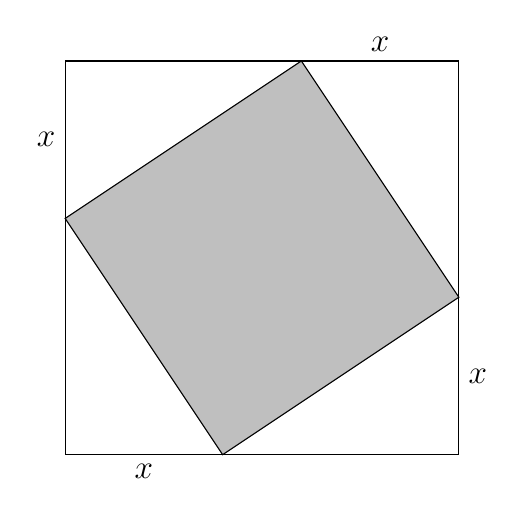
\begin{tikzpicture}
        \draw   (0,0) -- (5,0) -- (5,5) -- (0,5) -- cycle ;
        \draw  [fill={gray!50}] (2,0) -- (5,2) -- (3,5) -- (0,3) -- cycle ;
        \draw (5,1) node [right] {\large $x$};
        \draw (4,5) node [above] {\large $x$};
        \draw (0,4) node [left] {\large $x$};
        \draw (1,0) node [below] {\large $x$};
    \end{tikzpicture}
    \end{center}
\end{exer}

\begin{exer}
    Considere um quadrado com lado 4 cm como na figura.

    \begin{center}
    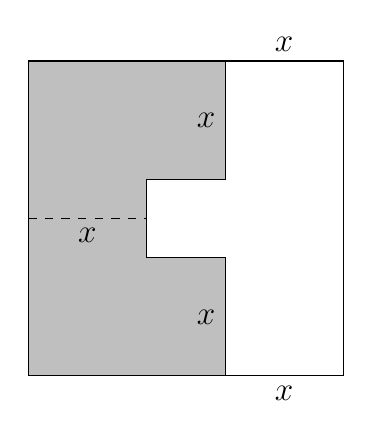
\begin{tikzpicture}
        \draw  [fill={gray!50}] (0,0) -- (2.5,0) -- (2.5,1.5) -- (1.5,1.5) -- (1.5,2.5) -- (2.5,2.5) -- (2.5,4) -- (0,4) -- cycle ;
        \draw   (0,0) -- (4,0) -- (4,4) -- (0,4) -- cycle ;
        \draw (3.25,4) node [above] {\large $x$};
        \draw (2.5,0.75) node [left] {\large $x$};
        \draw (2.5,3.25) node [left] {\large $x$};
        \draw (3.25,0) node [below] {\large $x$};
        \draw (0.75,2) node [below] {\large $x$};
        \draw  [dashed] (0,2) -- (1.5,2);
    \end{tikzpicture}
    \end{center}
    
    \begin{enumerate}[a)]
        \item Calcule $x$ (em cm) para que a área em destaque seja a maior possível;
        \item Calcule esta área.
    \end{enumerate}
\end{exer}
    
\end{secExercicios}